\documentclass[pdflatex,ja=standard]{bxjsarticle}

% Language setting
% Replace `english' with e.g. `spanish' to change the document language
\usepackage[japanese]{babel}
\usepackage{graphicx} % Required for inserting images
\usepackage{amsmath}
\usepackage{xeCJK}
\usepackage{listings}
\begin{document}
1.1 (a)

\begin{equation}
p(y) = \frac{1}{2} \cdot \frac{1}{\sqrt{2 \pi \cdot 2^2}} \exp{ \{ \frac{(y-1)^2}{2 \cdot 2^2} \}} + \frac{1}{2} \cdot \frac{1}{\sqrt{2 \pi \cdot 2^2}} \exp{ \{ \frac{(y-2)^2}{2 \cdot 2^2} \} }
\end{equation}

\begin{lstlisting}
#%%
import numpy as np
import matplotlib.pyplot as plt

def norm_dist(x: np.ndarray, mu: float, sigma: float) -> np.ndarray:
    return 1 / (sigma * np.sqrt(2 * np.pi)) * np.exp(- 1./2 * ((x - mu) / sigma) **2)

#%% 
x = np.linspace(-10, 10, 1000)
y1 = norm_dist(x, 1, 2)
y2 = norm_dist(x, 2, 2)

y = 1/2 * y1 + 1/2 * y2
plt.plot(x, y)
plt.show()

\end{lstlisting}

\begin{figure}
    \centering
    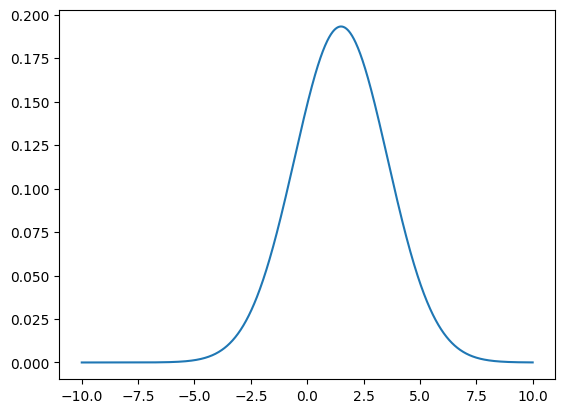
\includegraphics[width=0.5\linewidth]{norm_dist.png}
    \caption{1.1.(a) の描画結果}
    \label{fig:placeholder}
\end{figure}

1.1(b)
\begin{gather}
\rm{Pr} (\theta = 1 | y = 1) = \frac{Pr(\theta = 1) Pr(y=1 |\theta = 1) }{Pr(y=1)} \\
=  \frac{\exp(-\frac{(1-1)^2}{2 \cdot 2^2} ) }{\exp(-\frac{(1-1)^2}{2 \cdot 2^2}) + \exp(-\frac{(1-2)^2}{2 \cdot 2^2})} \\
= \frac{1}{1 + \exp(-0.125)} = 0.531
\end{gather}

1.1(c) \\
1.1(b)同様の式展開により、
\begin{gather}
\rm{Pr} (\theta = 1 | y) = \frac{\exp(-\frac{(y-1)^2}{2 \sigma^2} ) }{\exp(-\frac{(y-1)^2}{2 \sigma ^2}) + \exp(-\frac{(y-2)^2}{2 \sigma^2})} \\
= \frac{1}{1 + \exp(-\frac{-2y + 3}{2 \sigma^2})}
\end{gather}
$ f(x) = 1 / (1 +\exp(-\frac{x}{\sigma}))$ のグラフのスケールを変えて描画してみると、$\theta$の事後分布は$\sigma$が小さくなるほど0か1の両極端な分布となり、大きくなるほど $\rm{Pr} (\theta = 1|y) = \rm{Pr} (\theta = 2|y) = 0.5$ と偏りのない分布に近づくことがわかる。

\begin{lstlisting}
#%%
import numpy as np
import matplotlib.pyplot as plt

def func(x: np.ndarray, sigma: float) -> np.ndarray:
    return 1 / (1 + np.exp(-x / sigma))

#%% 
x = np.linspace(-10, 10, 1000)
y1 = func(x, 0.01)
y2 = func(x, 0.1)
y3 = func(x, 10)
y4 = func(x, 100)

plt.plot(x, y1, label="sigma=0.01")
plt.plot(x, y2, label="sigma=0.1")
plt.plot(x, y3, label="sigma=10")
plt.plot(x, y4, label="sigma=100")
plt.legend()
plt.show()
\end{lstlisting}

\begin{figure}
    \centering
    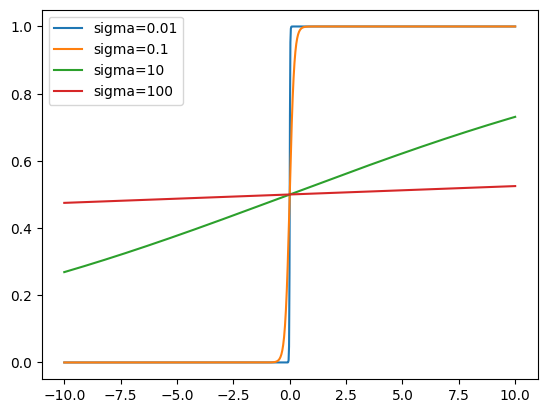
\includegraphics[width=0.5\linewidth]{output_sigmoid_like.png}
    \caption{1.1(c)の描画結果}
    \label{fig:placeholder}
\end{figure}

\end{document}
